\chapter{The Image Of Yourself}

This chapter follows J. Krishnamurti's Brockwood Park inquiry into the image of oneself, preserved from the Krishnamurti Foundation Trust source material and curated for this course by LazyingArt LLC through Video2Book. There are no validated blackboard equations or diagrammatic frames for this lecture, so the mathematics below is not recovered board work. It is a compact notation for the lecture's own distinctions: word and thing, conscious and ``unconscious,'' hurt and image, relationship and no relationship, method and fact. The notation is deliberately light, but it lets us keep track of the argument without smoothing away its pressure.

\section{The Unconscious As A Question}

The conversation resumes from the previous problem: human beings see the necessity of change, yet do not change. They accept, and in some sense maintain, intolerable conditions in the human psyche. Krishnamurti does not begin by adding another explanation. He proposes another angle.

The new angle is a question about the unconscious. But the word is not accepted as a settled technical term. It is put under pressure immediately. Who invented this unconscious? Who thought it up? Is the unconscious an actual movement of consciousness, or has the word already divided what is being observed?

The first useful notation is therefore almost anti-technical:

\begin{equation}
\text{word} \neq \text{thing}.
\end{equation}

This is not a slogan placed over the discussion. It is the first guardrail. If the word ``unconscious'' already carries the picture of a hidden chamber, then we may have accepted a structure before we have looked. One speaker gives the familiar account: there are aspects of experience of which one is incompletely aware; dreams may use symbols; slips of the tongue may reveal intention; past hurts may govern conduct without being explicitly known. Krishnamurti does not deny the phenomena too quickly. He questions the division.

Let us name the conventional picture as a layered model:

\begin{equation}
\mathcal{C}_{\text{surface}} \;+\; \mathcal{C}_{\text{hidden}}
\quad\text{with}\quad
\mathcal{C}_{\text{hidden}} = \text{``the unconscious''}.
\end{equation}

The discussion then asks whether that picture is already misleading. Perhaps there is not one conscious layer and another unconscious layer. Perhaps there is one movement of consciousness in which some fact is avoided, not because it belongs to a separate region, but because thought has learned not to face it.

\begin{equation}
\text{avoided fact} \;\not\Rightarrow\; \text{separate consciousness}.
\end{equation}

The distinction matters because a separated unconscious invites the language of digging, unearthing, exposing, lifting hidden contents out. Krishnamurti is asking whether the division itself is part of the fragmentation of the mind.

\subsection{Question \& Answer}

\paragraph{Question.}
Is the unconscious a separate layer of the psyche, or is it a name for facts avoided within one movement of consciousness?

\paragraph{Answer.}
The lecture does not simply erase the word. It uses it provisionally, almost in quotation marks. There are things not noticed, facts avoided, wounds not faced, habits of response whose origin is not clearly seen. But the stronger movement of the dialogue is away from a separate storehouse and toward fragmentation. The so-called unconscious may be what consciousness has put aside and then forgotten that it put aside.

\section{Fragmentation And The Wound That Remains}

Once the problem is stated this way, the next step is not to classify hidden contents. It is to examine avoidance. A disturbing fact is pushed away; the pushing away becomes habitual; eventually one may no longer know that one is avoiding. The wound is then not gone. It remains.

A compact reconstruction of this movement is:

\begin{align}
\mathcal{F}_{\text{disturbing}}
&\to \text{avoidance}, \\
\text{avoidance repeated}
&\to \text{habit}, \\
\text{habit}
&\to \text{forgetting that one has forgotten}, \\
\text{forgotten wound}
&\to \text{response from the past}.
\end{align}

Here \(\mathcal{F}\) denotes a fact, not a theory. The point is not that we have proved a psychological mechanism. The point is that the dialogue has shifted from an invisible chamber to an observable movement: one does not want to think about something because it hurts.

The speakers then sharpen this into a sequence. Being hurt brings resistance, withdrawal, isolation, and the picture of oneself as hurt and withdrawn. This is the first place where the image begins to enter the lecture as more than a word. Hurt is not merely an event. Hurt organizes a picture of oneself.

\begin{equation}
H \to \text{resistance} \to \text{withdrawal} \to \text{isolation} \to \mathcal{I}_{\text{hurt self}}.
\end{equation}

The symbol \(H\) denotes hurt or wound. The symbol \(\mathcal{I}\) denotes image. We use \(\mathcal{I}\) rather than \(I\), because the pronoun ``I'' is precisely what is in question.

A small feedback loop is already visible in the discussion. Hurt strengthens the image, and the image helps hide or preserve the hurt.

\begin{equation}
H \to \mathcal{I},
\qquad
\mathcal{I} \to \text{forgetting or concealing }H.
\end{equation}

This is not yet the whole argument. It is the point at which the inquiry becomes personal and exact. If hurt is one of the major wounds in human existence, must the psychological brain be hurt? Is hurt inevitable?

\section{The Image That Can Be Hurt}

The lecture's central move is simple and severe: what is hurt is the image of oneself. Most people, the speakers say, have an image about themselves. That image is not felt as an external possession. It is felt as ``me.'' Therefore an injury to the image is experienced as an injury to myself.

\begin{equation}
\mathcal{I}_{\text{self}} \equiv \text{``me''}.
\end{equation}

So the next equation follows in the lecture's own terms:

\begin{equation}
\text{injury to }\mathcal{I}_{\text{self}}
\Rightarrow
\text{``I am hurt.''}
\end{equation}

This is the decisive condensation. The image is not just a portrait hanging in the mind. It has been identified with the one who suffers. If someone contradicts it, punctures it, refuses to confirm it, or exposes it as false, the blow lands as personal pain.

The dialogue then adds an important symmetry. The image is attractive because it gives pleasure. I think I am good, clever, important, loved, chosen, secure, or admirable, and the pleasure is attributed to me. But the same mechanism that gives pleasure also makes pain possible. If the image can be confirmed, it can be contradicted. If it can be fed, it can be wounded.

\begin{align}
\mathcal{I}_{\text{self}} &\to P_{+}, \\
\mathcal{I}_{\text{self}} &\to P_{-},
\end{align}

where \(P_{+}\) denotes pleasure from the image and \(P_{-}\) denotes pain from the image. The paired implication is:

\begin{equation}
\text{pleasure from image}
\Rightarrow
\text{possibility of pain from image}.
\end{equation}

This is why the wish for an image that gives only pleasure is incoherent within the lecture's logic. One cannot keep the self-confirming image and be free from the wound that follows when the image is disturbed.

\subsection{Question \& Answer}

\paragraph{Question.}
Can the psychological brain never be hurt?

\paragraph{Answer.}
The answer is not given as a theory of the brain. The lecture keeps the distinction between physical shock and psychological hurt. Physical shock belongs to the organism. Psychological hurt, as explored here, requires reference to an image. If there is no image to be punctured, what is there to be hurt? The answer therefore turns on the image, not on a claim about biology.

\section{A Worked Example: The Pleasure-Pain Mechanism}

We can write the lecture's example as a small update rule. Suppose a child, or an adult, holds a self-image:

\begin{equation}
\mathcal{I}_{\text{self}}(t)
=
\text{``I am valued if I am this.''}
\end{equation}

Now let an event \(E_t\) either confirm or contradict that image. We do not use this as a psychological model; it is only a clean way to display the spoken logic.

\begin{align}
E_t = \text{confirmation}
&\Rightarrow
\mathcal{I}_{\text{self}}(t+1) = \mathcal{I}_{\text{self}}(t) + P_{+}, \\
E_t = \text{contradiction}
&\Rightarrow
\mathcal{I}_{\text{self}}(t+1) = \mathcal{I}_{\text{self}}(t) + P_{-}.
\end{align}

Here the plus sign means reinforcement or added charge, not numerical addition. The same image receives pleasure when it is confirmed and pain when it is contradicted. The result is that the image becomes increasingly important either way. Pleasure makes one invest in it; pain makes one defend it.

The derivation, in the lecture's order, is:

\begin{enumerate}
\item A self-image is formed and felt as ``me.''
\item Confirmation of the image gives pleasure.
\item Contradiction of the image gives pain.
\item Both pleasure and pain increase the importance of the image.
\item Therefore the mechanism cannot be arranged to yield pleasure only.
\end{enumerate}

This is also why hurt and image strengthen one another. The image is built partly to protect against hurt, yet because it can be hurt, it becomes the basis of further vulnerability.

\begin{equation}
H_{\text{past}} \to \mathcal{I}_{\text{stronger}} \to H_{\text{renewed}}.
\end{equation}

\section{Where Image-Making Begins}

The inquiry then moves backward. If the image is what gets hurt, where does the image begin? The transcript does not settle this by importing a developmental theory. It stages an argument.

One speaker proposes the child who learns that if he is smart, the father will like him. The child learns to become that. Krishnamurti presses further: what is the origin of making images about oneself at all? If a child had no image, would the father's action have the same psychological effect? If there is no image, what gets hurt?

The objection is practical and important. A child is vulnerable. A child needs physiological support, security, care. The discussion does not deny that. Instead it distinguishes biological fact from the psychological image made around the fact.

\begin{equation}
\text{biological dependence}
\neq
\text{psychological image of dependence}.
\end{equation}

The distinction is narrow but crucial. A child may need food, touch, shelter, order, and care. But the psychological wound under discussion belongs to the image: the image of being loved, not loved, approved, rejected, secure, abandoned, important, or unimportant.

The parent-child relation then becomes a field of transmission. If the parent has an image about himself or herself, the parent cannot fully see the child. The parent sees through image, acts from image, neglects through image, demands through image, and communicates image even when nothing explicit is taught.

\begin{equation}
\text{parent has }\mathcal{I}_{\text{self}}
\Rightarrow
\text{child receives or forms }\mathcal{I}_{\text{self}}.
\end{equation}

This is not presented as a universal scientific law. It is the dialogue's discovery: as long as the parent is an image-maker, the child is brought into an image-making field. Neglect itself communicates an image. Approval communicates an image. The steady building of image prepares the basis on which hurt can later occur.

Society enlarges the same movement. Family, school, religion, politics, culture, and nationality create images. One may change images, reject one image and take another, but the machinery remains.

\section{Relationship Or No Relationship}

The lecture's hardest relational claim comes next. If two people are related through images, is that relationship? Krishnamurti resists the softer phrase ``wrong relationship.'' He presses the distinction: relationship or no relationship.

We can write the two cases as:

\begin{align}
R_{\mathcal{I}} &= \text{relation governed by images}, \\
R_{\text{actual}} &= \text{relationship without image}.
\end{align}

The strong claim is:

\begin{equation}
R_{\mathcal{I}} \neq R_{\text{actual}}.
\end{equation}

And, in the lecture's sharper form:

\begin{equation}
\mathcal{I}_{\text{self}} \neq \varnothing
\Rightarrow
R_{\text{actual}} = \varnothing.
\end{equation}

This is not a theorem. It is a compact rendering of the claim being tested: as long as there is an image about oneself, one has no actual relationship with another.

The rope analogy makes the claim intelligible. A person may appear free within a certain range. He may say there are moments of relationship, moments of openness, moments in which nothing seems to interfere. But if he is tied to a rope, he is not free because he will eventually meet the limit. The image is that limit. At a certain point, it yanks the person back.

\begin{figure}
\centering
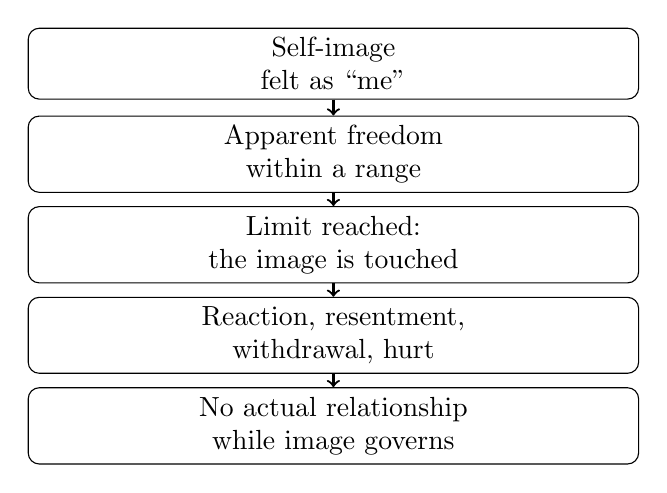
\begin{tikzpicture}[
  node distance=1.15cm,
  box/.style={draw, rounded corners, align=center, text width=0.62\linewidth, minimum height=0.8cm},
  smallbox/.style={draw, rounded corners, align=center, text width=0.42\linewidth, minimum height=0.7cm},
  arrow/.style={->, thick}
]
\node[box] (image) {Self-image\\felt as ``me''};
\node[box, below of=image] (range) {Apparent freedom\\within a range};
\node[box, below of=range] (limit) {Limit reached:\\the image is touched};
\node[box, below of=limit] (yank) {Reaction, resentment,\\withdrawal, hurt};
\node[box, below of=yank] (norel) {No actual relationship\\while image governs};

\draw[arrow] (image) -- (range);
\draw[arrow] (range) -- (limit);
\draw[arrow] (limit) -- (yank);
\draw[arrow] (yank) -- (norel);
\end{tikzpicture}
\end{figure}

The lecture is careful here. A participant admits resentment at the claim, precisely because there are memories of what seemed to be relationship. But the rope image clarifies the point. If the image takes over beyond a certain point, then the image has been the governing factor all along. The moments were real as moments, but not freedom from the mechanism.

\section{Can The Machinery Stop?}

The final movement gathers the inquiry into one question. The image is a major content of consciousness, perhaps the major machinery operating in it. The content of consciousness makes up consciousness, and one of its central contents is image-making.

\begin{equation}
\mathcal{C} = \text{content of consciousness},
\qquad
\mathcal{I} \subset \mathcal{C}.
\end{equation}

The machinery is then identified more directly:

\begin{equation}
\text{image-making} = \text{product of thought}.
\end{equation}

Thought produces images: religious images, national images, images of status, images of being chosen, images of being nobody, images of having to become somebody. These images divide. Division destroys relationship. Without relationship, love becomes verbal, sentimental, fanciful, or romantic, but not actual.

\begin{equation}
\text{thought} \to \text{image} \to \text{division} \to \text{no love}.
\end{equation}

So the question becomes unavoidable: can this image-making stop? Not occasionally. Not for a moment before returning. Can the machinery stop?

\subsection{Question \& Answer}

\paragraph{Question.}
How can image-making stop?

\paragraph{Answer.}
The lecture refuses the word ``how'' at the decisive point. A how would become method, system, practice, and another image. Evidence, experience, explanation, and future promise are also refused because each can become an image: past image, future image, living image.

The proposed movement is not a technique. It is to see the fact and remain with the fact, without thought adding commentary.

\begin{align}
\mathcal{F} + \text{thought/commentary}
&\to \mathcal{I}_{\text{new}}, \\
\mathcal{F} + \text{no commentary}
&\to \text{transformation}.
\end{align}

The word ``transformation'' should not be treated as an operator or a result one can manufacture. It names what the lecture says occurs when the mind remains with the fact without running away into another image.

\begin{figure}
\centering
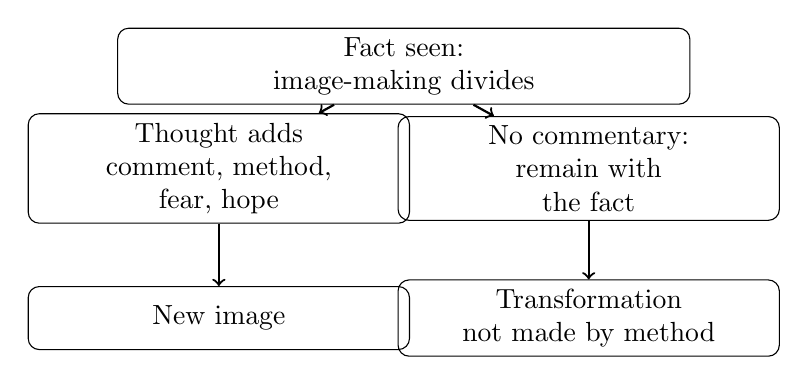
\begin{tikzpicture}[
  node distance=1.2cm,
  box/.style={draw, rounded corners, align=center, text width=0.58\linewidth, minimum height=0.8cm},
  side/.style={draw, rounded corners, align=center, text width=0.38\linewidth, minimum height=0.8cm},
  arrow/.style={->, thick}
]
\node[box] (fact) {Fact seen:\\image-making divides};
\node[side, below left of=fact, xshift=-1.5cm, yshift=-0.45cm] (comment) {Thought adds\\comment, method,\\fear, hope};
\node[side, below right of=fact, xshift=1.5cm, yshift=-0.45cm] (stay) {No commentary:\\remain with\\the fact};
\node[side, below of=comment, yshift=-0.7cm] (newimage) {New image};
\node[side, below of=stay, yshift=-0.7cm] (trans) {Transformation\\not made by method};

\draw[arrow] (fact) -- (comment);
\draw[arrow] (fact) -- (stay);
\draw[arrow] (comment) -- (newimage);
\draw[arrow] (stay) -- (trans);
\end{tikzpicture}
\end{figure}

The closing has a distinctive restraint. The lecture does not end by explaining what consciousness is without image-making. It leaves that as the next question. If consciousness is filled with images, conclusions, ideas, and running away, then what is consciousness when image-making is absent? That question is not answered here. It is opened.

\section{Summary}

The lecture begins by questioning the unconscious and ends by questioning consciousness itself. The movement is continuous. What is called unconscious may not be a separate layer but avoided fact within a fragmented mind. Avoidance leaves the wound in place. The wound leads to resistance, withdrawal, and the image of oneself as hurt. The image is then seen as the thing that can be pleased and hurt, because it is felt as ``me.''

From there the inquiry widens: parents, children, society, religion, politics, and culture all participate in image-making. Where image governs, relationship is not actual relationship. The image gives apparent range, but like a rope, it eventually limits and yanks back. The machinery behind it is thought. The final question is whether that machinery can stop. The lecture's answer is not a method but a demand for direct perception: see the fact of image-making and remain with it without turning it into another image.